Um die Funktionen im Frontend mit den benötigten Daten zu beliefern, wurden für das Backend drei Azure Functions erstellt, welche mit HTTP-Requests aufrufbar sind. Dazu wurde ein NER-Modell mithilfe von einem Notebook konfiguriert und antrainiert.

\subsection{NER-Modell}

spaCy ist die marktführende Technologie im Bereich NLP und bietet die Möglichkeit an ein eigenes NER-Modell anzutrainieren. Um dieses Modell anzutrainieren, müssen die Daten einem bestimmten Format entsprechen. Dieses Format entspricht einem Array, welches aus Tuples besteht. Das erste Element ist der Text und das zweite ist die dazugehörigen Entitäten mit Startindex und Endindex.

\begin{lstlisting}[language=Python, caption={Beispiel für ein Array mit Trainingsdaten}]
    [
        ("Tokyo Tower is 333m tall.", [(0, 11, "BUILDING")]),
    ]   
\end{lstlisting}

Um die vom Frontend exportierten Felder verarbeiten zu können, müssen sie zuerst in dieses Format gebracht werden. Dafür wird zunächst der Text aus der dazugehörigen Rechnung ausgelesen. Als Nächstes wird für jede Entität der Startindex und Endindex ausgelesen, wobei hier zu beachten ist, dass von \gls{ocr} erkannter Text nicht immer zu 100\% stimmt. Daher wurden drei Rückfallmethoden eingebaut.

\begin{enumerate}
    \item Der Inhalt der Entität wird genau wie angegeben im Text gesucht.
    \item Der Inhalt der Entität wird genau wie angegeben im Text gesucht, jedoch darf ein Zeichen unterschiedlich sein.
    \item Der Inhalt der Entität wird genau wie angegeben im Text gesucht, jedoch werden manche Zeichen mit ähnlich aussehenden Zeichen ausgetauscht. 
\end{enumerate}

\begin{minipage}{\linewidth}
\begin{lstlisting}[caption={Rückfallmethode 3}, label={search_with_similar_chars}]
    def search_with_similar_chars(str, text, entity):
        temp_value = ''
        for i in range(0,len(str)):
            similar_chars = similar_looking_chars(str[i])
            if similar_chars:
                temp_value += '('+'|'.join(similar_chars)+')'
            else:
                temp_value += str[i]
        catch_total = re.search(temp_value, text)
        if catch_total != None:
            ent_tup = (catch_total.span()[0], catch_total.span()[1], entity)
            return ent_tup
\end{lstlisting}
\end{minipage}

Wie in Listing \ref{search_with_similar_chars} zu sehen ist, wird mit Regex gearbeitet, was die Suche um einiges vereinfacht. Dabei wird auf den Operator ''|'' zurückgegriffen, durch den man mehrere unterschiedliche Zeichen für einen einsetzen kann.

Neben den vorgegebenen Entitäten gehören noch die Tabellen-Header zu den verpflichtenden Entitäten, da diese später für die Tabellenextraktion benötigt wird. 

\begin{lstlisting}[caption={Verpflichtende Entitäten}]
    field_names = {'company-name', 'company-address', 'invoice-id', 'invoice-date', 'total-value', 'item-header', 'qty-header', 'rate-header', 'total-header'}
\end{lstlisting}

Nachdem die Trainingsdaten im richtigen Format sind, kann das Modell antrainiert werden. Dafür wird ein leeres spaCy-Modell geladen und alle Entitäten werden hinzugefügt. Zur Kontrolle wird noch zusätzlich überprüft, ob der Startindex und Endindex wirklich eine vollendete Wortgruppe angeben. Falls dies nicht der Fall ist, wird die Entität übersprungen. Am Ende wird das Modell in einen Ordner exportiert, welches vor der Nutzung noch fertig trainiert werden muss.

\begin{lstlisting}[caption={Trainieren vom Modell}]
    nlp = spacy.blank("en")
    doc_bin = DocBin() 

    for training_example in training_data: 
        text = training_example['text']
        labels = training_example['entities']
        doc = nlp.make_doc(text) 
        ents = []
        for start, end, label in labels:
            span = doc.char_span(start, end, label=label, alignment_mode="contract")
            if span is None:
                print("Skipping entity", label)
            else:
                ents.append(span)
        filtered_ents = filter_spans(ents)
        doc.ents = filtered_ents 
        doc_bin.add(doc)

        doc_bin.to_disk("model/training_data.spacy")
\end{lstlisting}

\subsubsection{Utils}

Um Codewiederholung zu vermeiden und ähnliche Funktionen zu gruppieren, wurden drei UtilsKlassen erstellt, die später in den Azure Functions aufgerufen werden.

\paragraph{BoundingBoxes}

Diese UtilsKlasse erkennt jegliche Boxen, welche eine Wortgruppe umranden und gibt diese an den Aufrufer zurück.

Dafür wird zuerst mithilfe von \lstinline{pytesseract} für jedes Wort oder jede Zahl eine Box gespeichert. Jedoch werden dadurch zusammengehörige Wortgruppen voneinander getrennt. Um diese zu verbinden, werden zuerst alle Wörter nach Zeilen gruppiert und durchiteriert. Dabei wird der horizontale Abstand zwischen den Boxen berechnet und liegt dieser Wert unter einem gewissen Wert, werden diese zwei Boxen miteinander verbunden.

\begin{lstlisting}[caption={Syntax um zusammengehörige Wortgruppen zu verbinden}]
    def __merge(self, boxes, dist_limit = 10, cell_threshold=50):
        rows = self.__get_rows(boxes, cell_threshold)
        for row in rows.values():
            i=0
            while i<len(row)-1:
                if self.__calc_horizontal_distance(row[i], row[i+1]) <= dist_limit:
                    row[i] = self.__merge_boxes(row[i], row[i+1])
                    row.pop(i+1)
                else:
                    i += 1
        return [item for sublist in list(rows.values()) for item in sublist]
\end{lstlisting}

\paragraph{Text}

Diese UtilsKlasse extrahiert den Text eines Bildes sowohl formatiert als auch unformatiert. Dabei nutzen beide Funktionen pytesseract, um den Text zu lesen und jegliche Informationen zur Position zu gewinnen. Der einzige Unterschied ist, dass der Text auf eine andere Weise aufbereitet wird.

\begin{figure}[H]
    \centering
    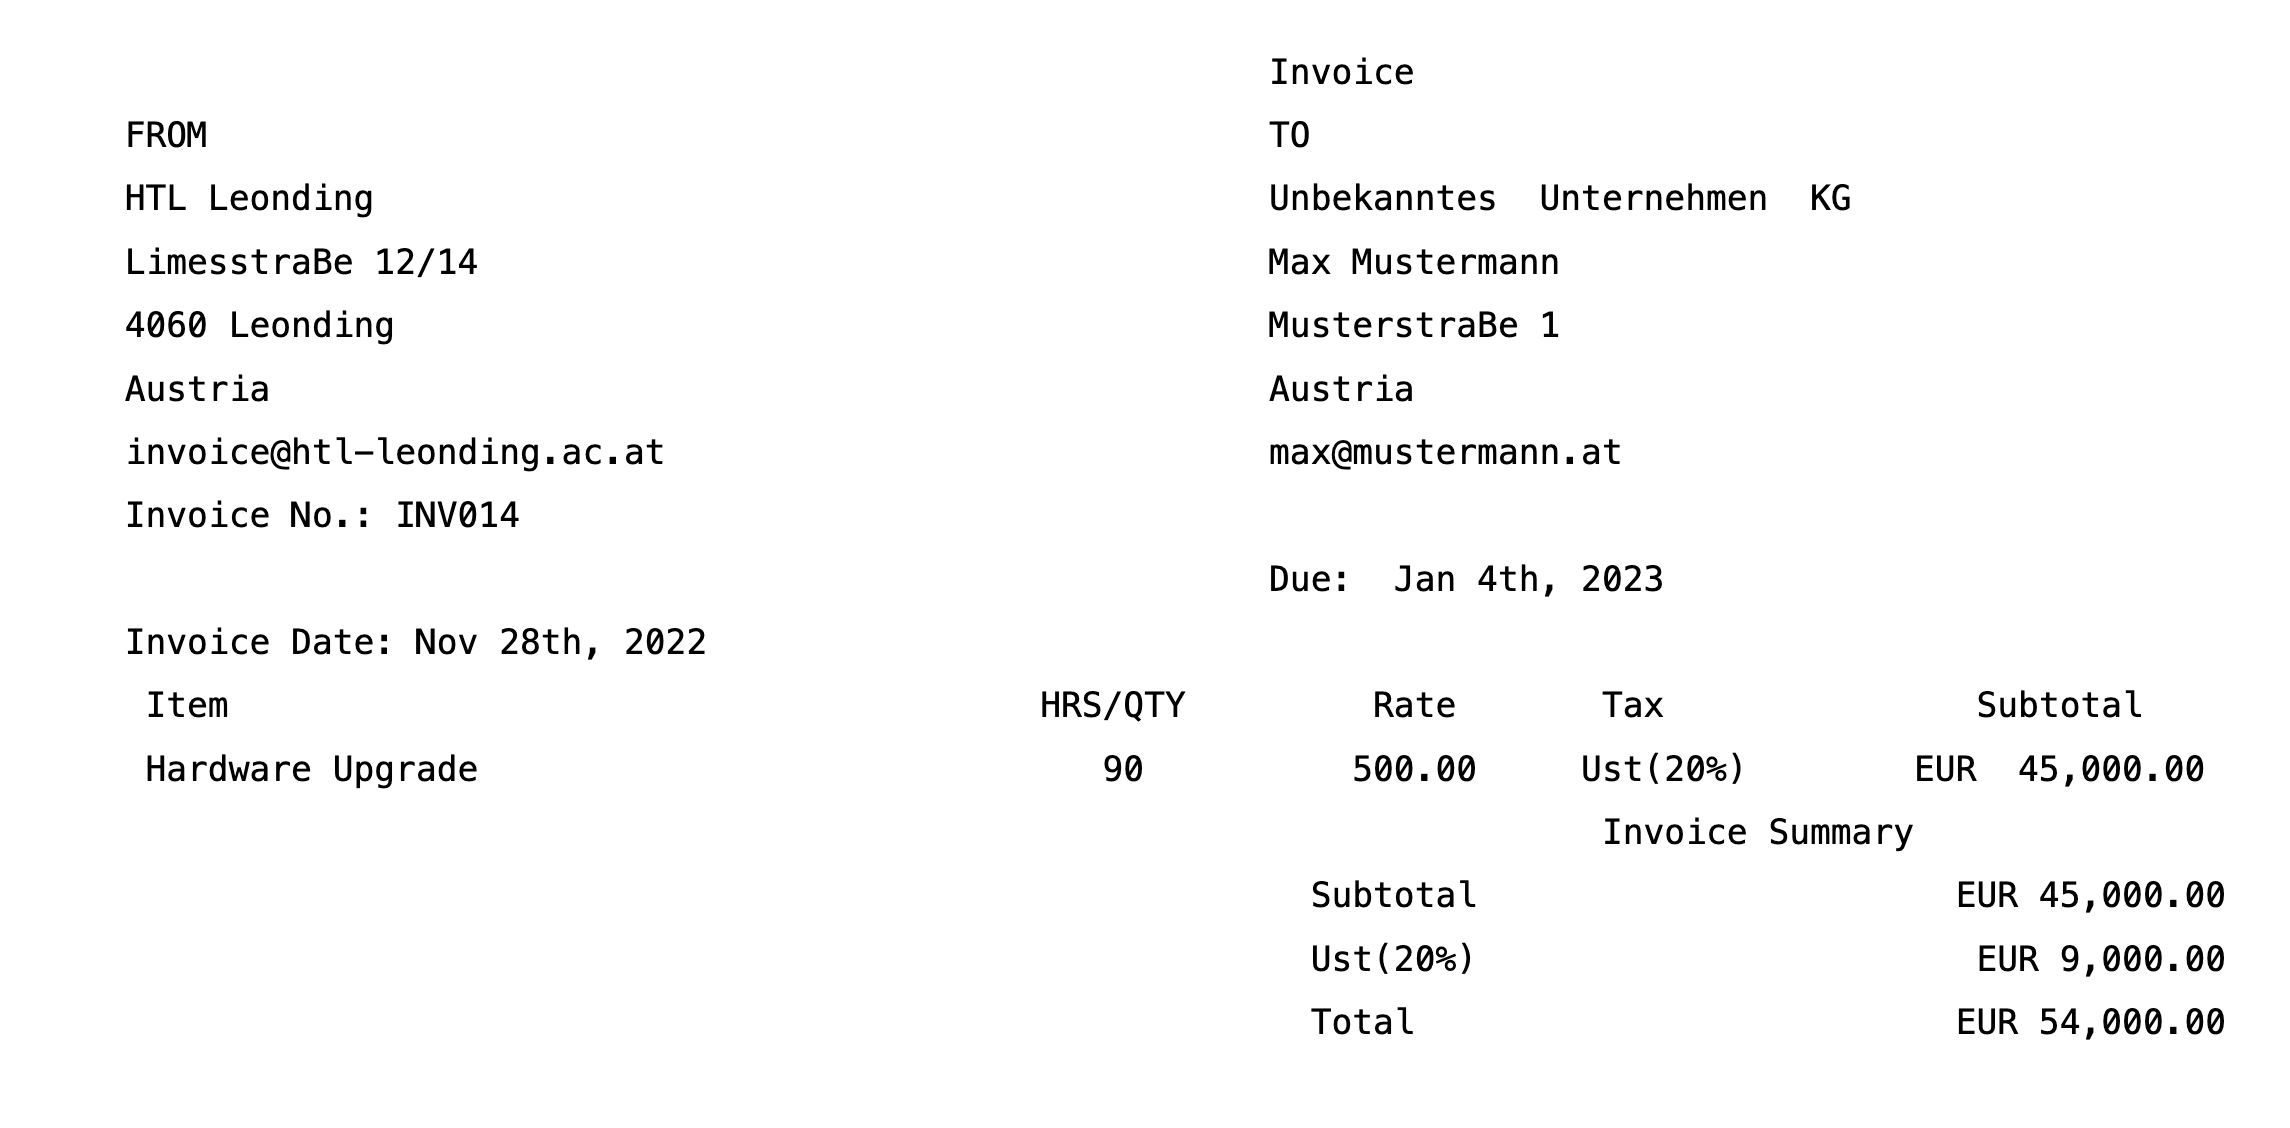
\includegraphics[scale=0.3]{sections/implementation/images/formated.png}
    \caption{Beispiel für einen formatierten Text}
\end{figure}

\begin{figure}[H]
    \centering
    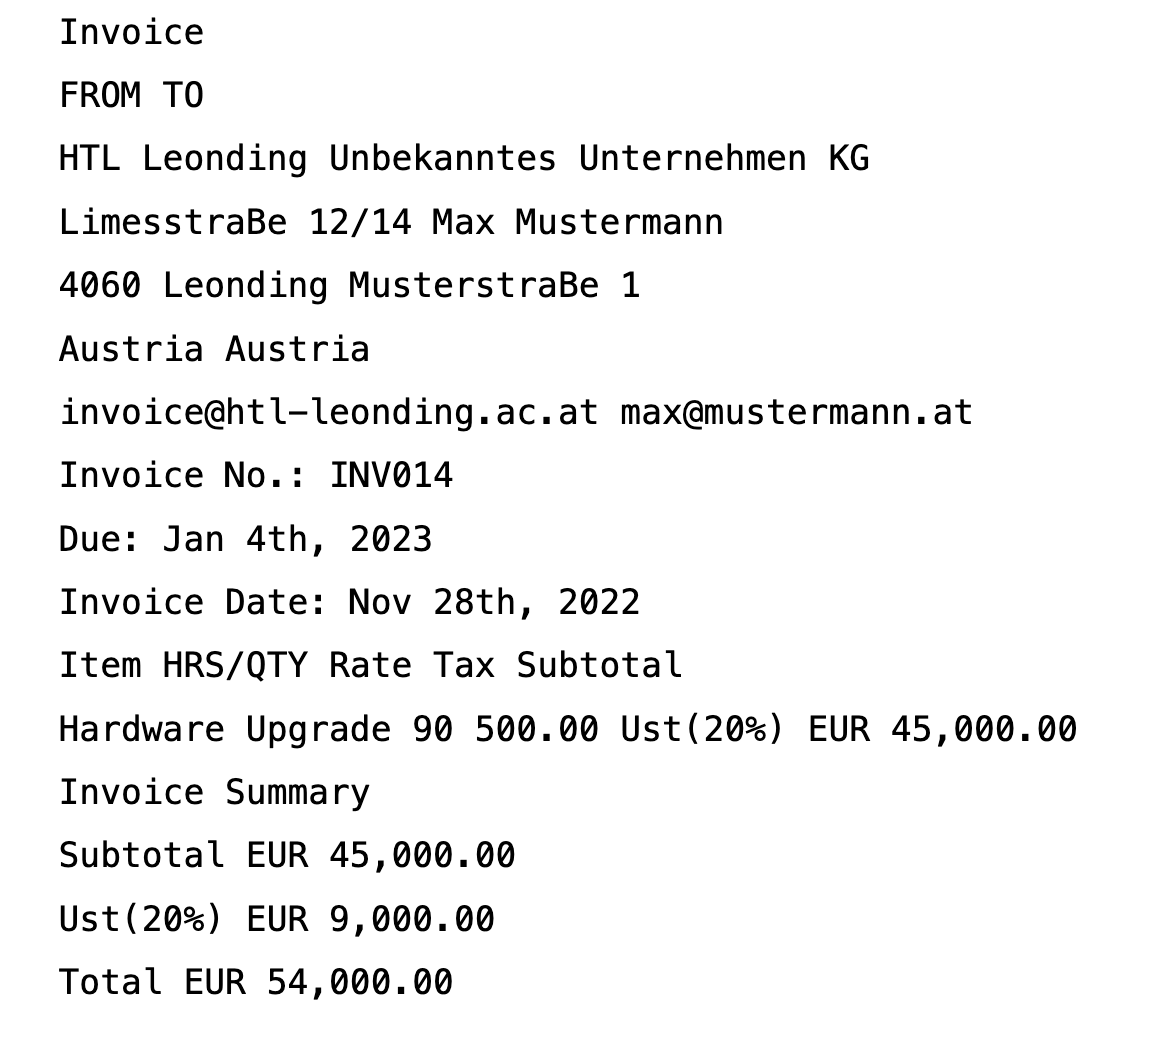
\includegraphics[scale=0.4]{sections/implementation/images/unformated.png}
    \caption{Beispiel für einen unformatierten Text}
\end{figure}

Wie in den überliegenden Abbildungen zu sehen ist, befindet sich der Text in der gleichen Reihenfolge und der einzige Unterschied liegt im Abstand zwischen den Wörtern.

\paragraph{InvoiceData}

Diese UtilsKlasse extrahiert aus einem übergebenen Text die vorgegebenen Entitäten und Rechnungszeilen. Dafür ist sie in zwei Schritte unterteilt.

\subparagraph{Entität Extrahierung} 

Mithilfe vom davor antrainiertem NER-Modell wird der Text verarbeitet und alle Entitäten werden in einem Dictionary gespeichert. 

\begin{lstlisting}[caption={Extrahierung von Entitäten}]
    nlp_ner = spacy.load(modelPath)
    doc = nlp_ner(text)
    for ent in doc.ents:      
        op_dict[ent.label_] = ent.text
\end{lstlisting}

\subparagraph{Tabellen Extrahierung}

Mit dem davor extrahierten Tabellen-Header wird die Tabellen-Header Zeile bestimmt und der formatierte Text wird bis zur dieser Zeile gekürzt. Mithilfe von pandas kann der übrig gebliebene Text in ein Dataframe umgewandelt werden. 

\begin{minipage}{\linewidth}
\begin{lstlisting}[caption={Tabellen Extrahierung}]
    header_row = max(set(header_rows), key=header_rows.count)
    table = formatted_text_lines[header_row:]
    text = '\n'.join(table)

    df = pd.read_csv(StringIO(text), sep='\s{3,}', engine='python', index_col=False).dropna()
    
    items = []
    for i in range(0, df.shape[0]):
        item = {}
        for header_field in header_fields:
            item[op_dict.get(header_field)] = df.loc[i][op_dict.get(header_field)]
        items.append(item)
    op_dict['items'] = items
\end{lstlisting}
\end{minipage}

\subsubsection{Azure Functions}

Um die in Utils definierten Methoden im Frontend aufrufen zu können, wurden sie als Azure Functions zusammengefasst. Das Resultat sind drei über einen HTTP-Request aufrufbare Funktionen.

Genau wie die Utils-Klassen wurden die Azure Functions mit der Skriptsprache Python entwickelt. Zusätzlich wurde die Visual Studio Code Erweiterung für Azure Functions genutzt, um diese zu generieren und zu konfigurieren.

Jede Azure Function besteht aus einer Konfigurationsdatei und einer Datei, welche den eigentlichen Code beinhaltet. Dabei gibt die Konfigurationsdatei das Authentifizierungsmittel, die erlaubten HTTP-Methoden und die Auslöseart an. Im unterliegenden Listing wird die Azure Function zum Beispiel mithilfe von einem POST-HTTP-Request ausgelöst.

\begin{lstlisting}[caption={Beispiel fuer eine Konfigurationsdatei}]
    {
        "scriptFile": "__init__.py",
        "bindings": [
            {
                "authLevel": "function",
                "type": "httpTrigger",
                "direction": "in",
                "name": "req",
                "methods": [
                    "post"
                ]
            },
            {
                "type": "http",
                "direction": "out",
                "name": "\$return"
            }
        ]
    }
\end{lstlisting}

Die drei Azure Functions wurde jeweils so aufgeteilt, dass sie eine bestimmte Aufgabe erfüllen. 

\paragraph{Bounding Box}

Wie der Name sagt werden die Bounding Boxes von dieser Azure Function generiert. Dafür wird zuerst das Bild im Byte-Format aus dem HTTP-Request-Body in ein von Python verarbeitbares Image umgewandelt. Als Nächstes wird die Utils-Klasse initialisieren und zum Generieren der BoundingBoxes genutzt. 

Das Result wird in einem HTTP-Response-Body zurückgegeben, dabei hat der Request den Response Code 200, welcher angibt, dass der Request erfolgreich durchgeführt wurde. 

In zwei Situationen werden Response Codes zurückgegeben, die in­di­zie­ren, dass der Request nicht fehlerfrei umgesetzt wurde. Diese Wären:

\begin{enumerate}
    \item Falls der HTTP-Request-Body leer ist, wird ein Response Code von 400 zurückgegeben, der angibt, dass der HTTP-Request nicht valide aufgebaut ist.
    \item Falls beim Generieren ein Fehler auftritt, wir ein Response Code von 500 zurückgegeben, der angibt, dass serverseitig ein Fehler aufgekommen ist.
\end{enumerate}

\paragraph{Size}

Da das Frontend die pdf-Datei in einer abweichenden Grüße darstellt, wird die Originalgröße benötigt, um die Bounding Boxen auf der richtige Position darzustellen. Diese Bildgröße wird in einem Tuple zurückgegeben. 

Die Response Codes sind ident zu den von der Bounding Box Azure Function.

\paragraph{Invoice Data} 

Damit das Modell von außen erreichbar ist, dient diese Azure Function als Schnittstelle. Beim Aufruf der Methode besteht die Möglichkeit, den Pfad zum gespeicherten Modell anzugeben. Da spaCy sowohl das präziseste als auch das in der letzten Iteration erstellte Modell speichert, hat man die Möglichkeit zwischen eines der beiden zu entscheiden. Normalerweise sollte das präziseste Modell genutzt werden, da man mit diesem Modell auch das beste Ergebnis erhaltet.

\begin{minipage}{\linewidth}
\begin{lstlisting}[caption={Invoice Data Azure Function}, label={invoiceData}]
    def main(req: func.HttpRequest) -> func.HttpResponse:
        try:
            logging.info('Invoice data registered a request.')
            
            body = req.get_body()
            pages = convert_from_bytes(body)
            image = np.array(pages[0])

            logging.info('Bytes have been successfully converted into a Image.')

            if body:
                invoice_data = InvoiceData()

                logging.info('InvoiceData class has been initialized.')

                data = invoice_data.get_invoice_data(image, 'model/model-best')

                logging.info('Invoice data has been successfully read.')

                return func.HttpResponse(json.dumps(data), mimetype="application/json")
            else:
                return func.HttpResponse('Request does not contain a body.', status_code=400)
        except Exception as e:
            logging.exception(e)
            return func.HttpResponse("An error occurred while processing the request", status_code=500)
\end{lstlisting}
\end{minipage}

Wie man im Listing \ref{invoiceData} sieht, werden die wichtigsten Informationen mithilfe von einem Logger ausgegeben. Dies hilft beim Auftreten von einem Fehler, dass dieser Fehler schnellstmöglich lokalisiert und behoben wird.